\documentclass[a4paper,11pt]{article}
\usepackage{lscape}
\usepackage{a4wide}		%wider margins for a4 paper
\usepackage{amssymb}
\usepackage{amsmath}
\usepackage{graphicx}
\usepackage{url}
\usepackage{hyperref}	%automatic links to sections, figures, references
\usepackage[all]{hypcap}%links to top of figures
\usepackage{soul}		%highlighting with \hl{}
\usepackage{color}		%color, also color highlighting
\usepackage{xcolor}
\usepackage{setspace}	%line spacing
\usepackage{multirow}	%multirow and multicolumn cells in tables
\usepackage{subfig}		%\subfloat in figures
\usepackage{multicol}
\usepackage{paracol}
%\usepackage[version=3]{mhchem}		%\ce{} for chemical formulae
\usepackage{wrapfig}	%\begin{wrapfigure}
\usepackage{lscape}
\usepackage{enumerate}
\usepackage[toc,page]{appendix}
\usepackage[final]{pdfpages}
\usepackage{amsfonts}              % for blackboard bold, etc
\usepackage{amsthm}                % better theorem environments
\usepackage{tabularx}
\usepackage{array}
\usepackage{listings} 
\usepackage{enumerate,letltxmacro}
\LetLtxMacro\itemold\item
\renewcommand{\item}{\itemindent1.5cm\itemold}
\usepackage[none]{hyphenat}

\title{MCB 5430 midterm assignment}
\author{Bianca Mocanu}

%header
\usepackage{fancyhdr}
\pagestyle{fancy}
\fancyhead[R]{MCB 5430 midterm}
\fancyhead[L]{Bianca Mocanu}
\cfoot{\thepage}
% -- 
%-------------


\lstset{
  basicstyle=\ttfamily,
  columns=fullflexible,
  frame=single,
  breaklines=true,
  postbreak=\mbox{\textcolor{red}{$\hookrightarrow$}\space},
}

\begin{document}

\begin{titlepage}

\begin{center}
\noindent \Large{\textbf{MCB 5430 midterm assignment}}\\
\vspace{0.7cm}
\small{Bianca Mocanu}\\

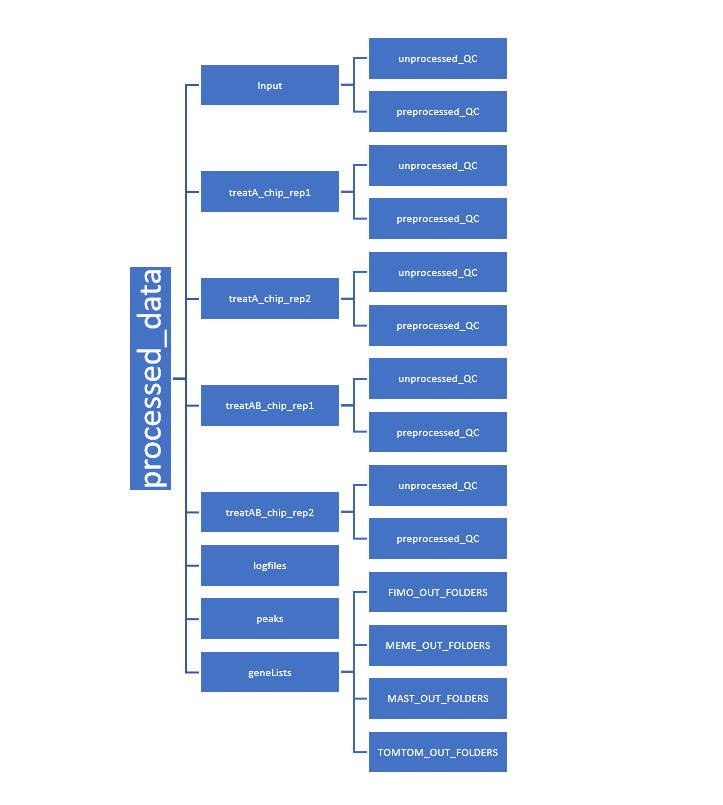
\includegraphics[scale=1]{folder_tree.PNG}
\noindent \footnotesize Tree folder structure of the script output
\end{center}
\end{titlepage}

\section{ChIP-seq processing, alignment and display}
\subsection{Pipeline}
\normalsize The shell script used in processing all of the data in this midterm can be found \color{blue}\href{https://github.com/biancamocanu/MCB5430_midterm/blob/master/pipe.sh}{here}. \color{black}

\subsection{Summary table}

\noindent The mapping of the reads has been done with the -m 1 option. Therefore, the "reads with at least one reported alignment" field in the log file refers to the number of uniquely mapped reads that fulfilled the mapping parameters. Table 1 displays the summary of the reads alignment step of the pipeline.\\

\footnotesize

\textbf{Table 1.} Summary table for the alignment step of the pipeline. Reads total refers to the number of fastq reads that passed the preprocessing steps of the pipeline. "\# and \% unique" display the number and the percentage of uniquely mapped reads. "\# and \% multiple" display the number and the percentage of multiply mapped reads that got discarded due to the constrains of the mapping parameter -m 1. "\# and \% unaligned" display the number and percentage of reads that did not align to the hg19 genome.
\begin{flushright}
\begin{tabular}{|p{1.6cm}|p{1.8cm}|p{1.8cm}|p{1.8cm}|p{1.8cm}|p{1.2cm}|p{1.2cm}|p{1.2cm}|}
 \hline 
 Sample & \# reads total & \# unique & \# multiple & \# unaligned & \% unique & \% multiple & \% unaligned \\ 
 \hline 
 Input & 12,265,901 & 10,088,192 & 1,016,900 & 1,160,809 & 82.25 & 8.29 & 9.46 \\ 
 \hline 
 treatment A rep 1 & 13,164,770 & 10,716,882 & 921,317 & 1,526,571 & 81.41 & 7.00 & 11.60 \\ 
 \hline 
 treatment A rep 2 & 14,071,793 & 11,248,659 & 971,196 & 1,851,938 & 79.94 & 6.90 & 13.16 \\ 
 \hline 
 treatment AB rep 1 & 13,132,269 & 10,686,406 & 955,345 & 1,490,518 & 81.38 & 7.27 & 11.35 \\ 
 \hline 
 treatment AB rep 2 & 8,725,137 & 6,948,241 & 601,088 & 1,175,808 & 79.63 & 6.89 & 13.48 \\ 
 \hline 
 \end{tabular}  

\end{flushright} 
 \normalsize

\section{Genome browser shot}
The genome browser PDF document displays the highest peak on Chromsome 12 and can be found \color{blue}\href{https://github.com/biancamocanu/MCB5430_midterm/blob/master/hgt_genome_64f1_bc6f0.pdf}{here}. \color{black} 
\pagebreak

\section{Peak calling and analysis}
\noindent The following part of the script includes the peak calling step, high confidence peak files generation and getting the peaks unique to each treatment. Since they were all typed in a single for loop, they are displayed together below (therefore the for loop ends on next page).
\subsection{MACS}
\noindent 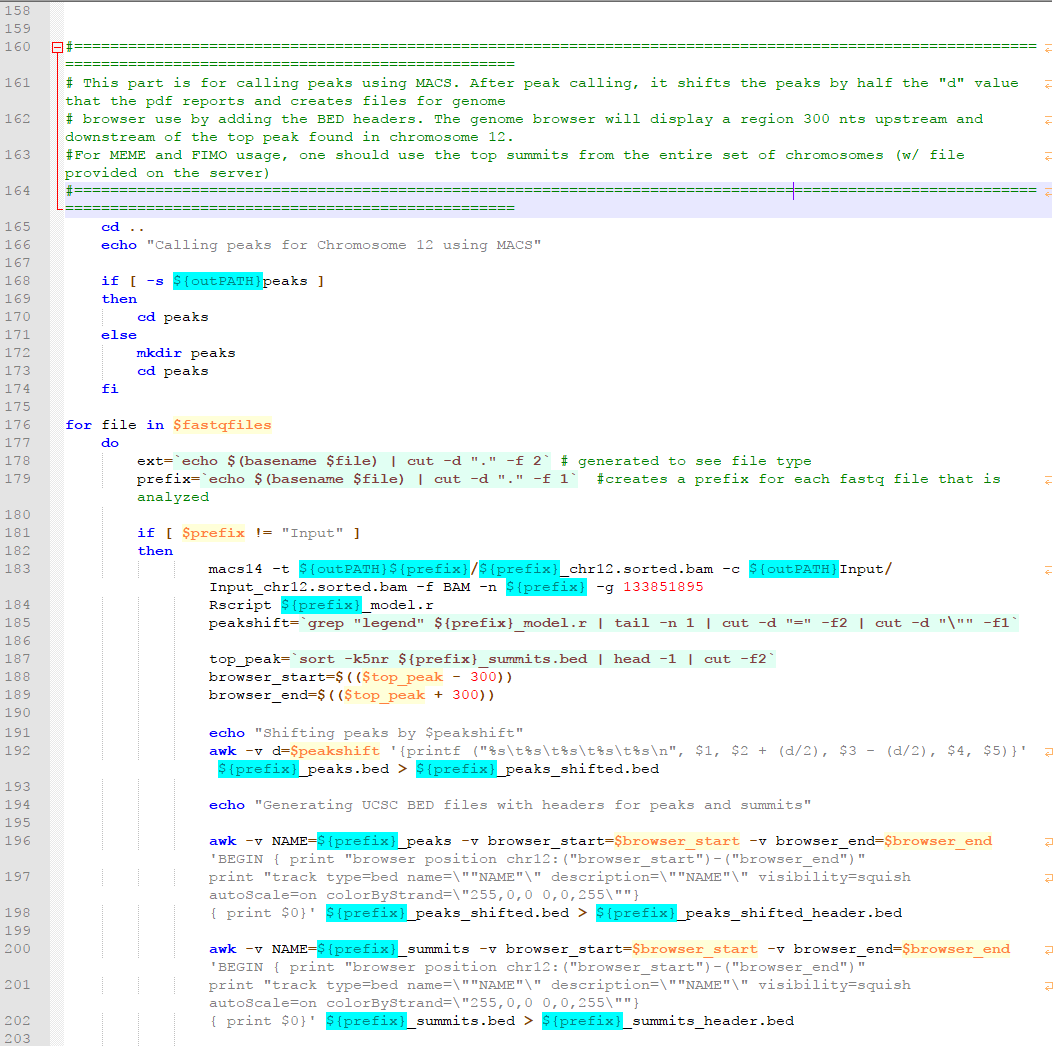
\includegraphics[scale=0.75]{MACS1.PNG}
\pagebreak
\subsection{High confidence peaks and 2.3 Peaks specific to each treatment}
\noindent 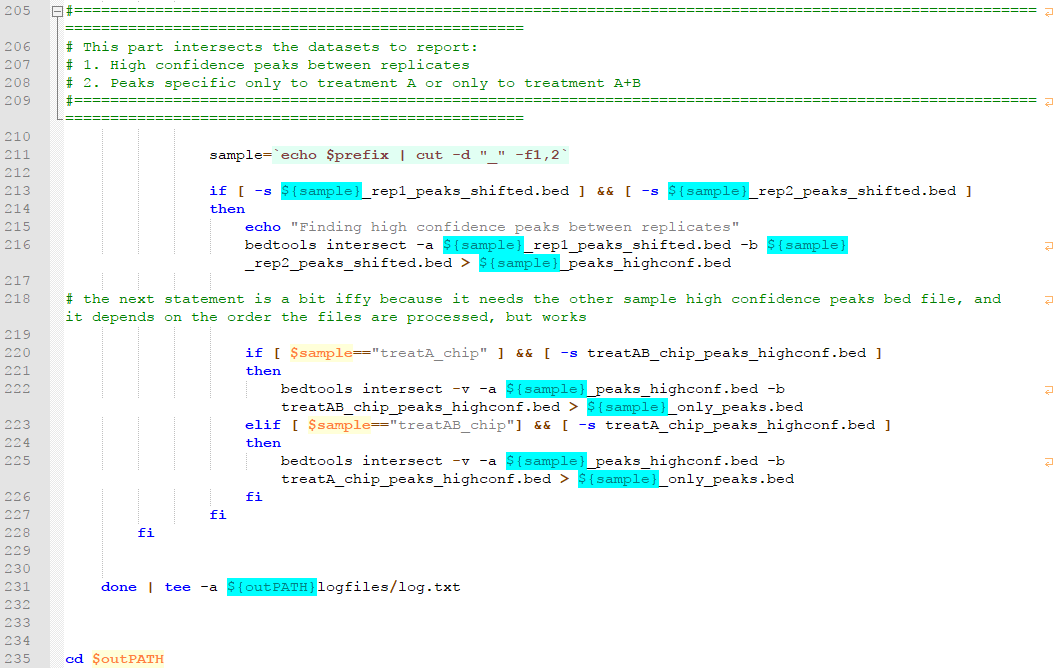
\includegraphics[scale=0.75]{MACS2.PNG} \\


\noindent \textbf{Observation:} The file containing peaks unique to treatment AB only is an empty file. This does not seem to be a script error - upon analysis of the peaks common to both treatments and peaks unique to treatment A, it is likely that AB peaks are a subset of A peaks. This already might mean that whatever treatment AB is, it inhibits the binding of this transcription factor to DNA.

\section{Distribution of TF binding sites}
\subsection{Bed files with promoter, gene and intergenic sequences}
\noindent For this step, TSS abbreviation of the files stands for the promoters, genes represent the genes and IGS represent the intergenic sequences. In addition to .bed files for each region type, .fasta files have been created here as well.\\

\noindent 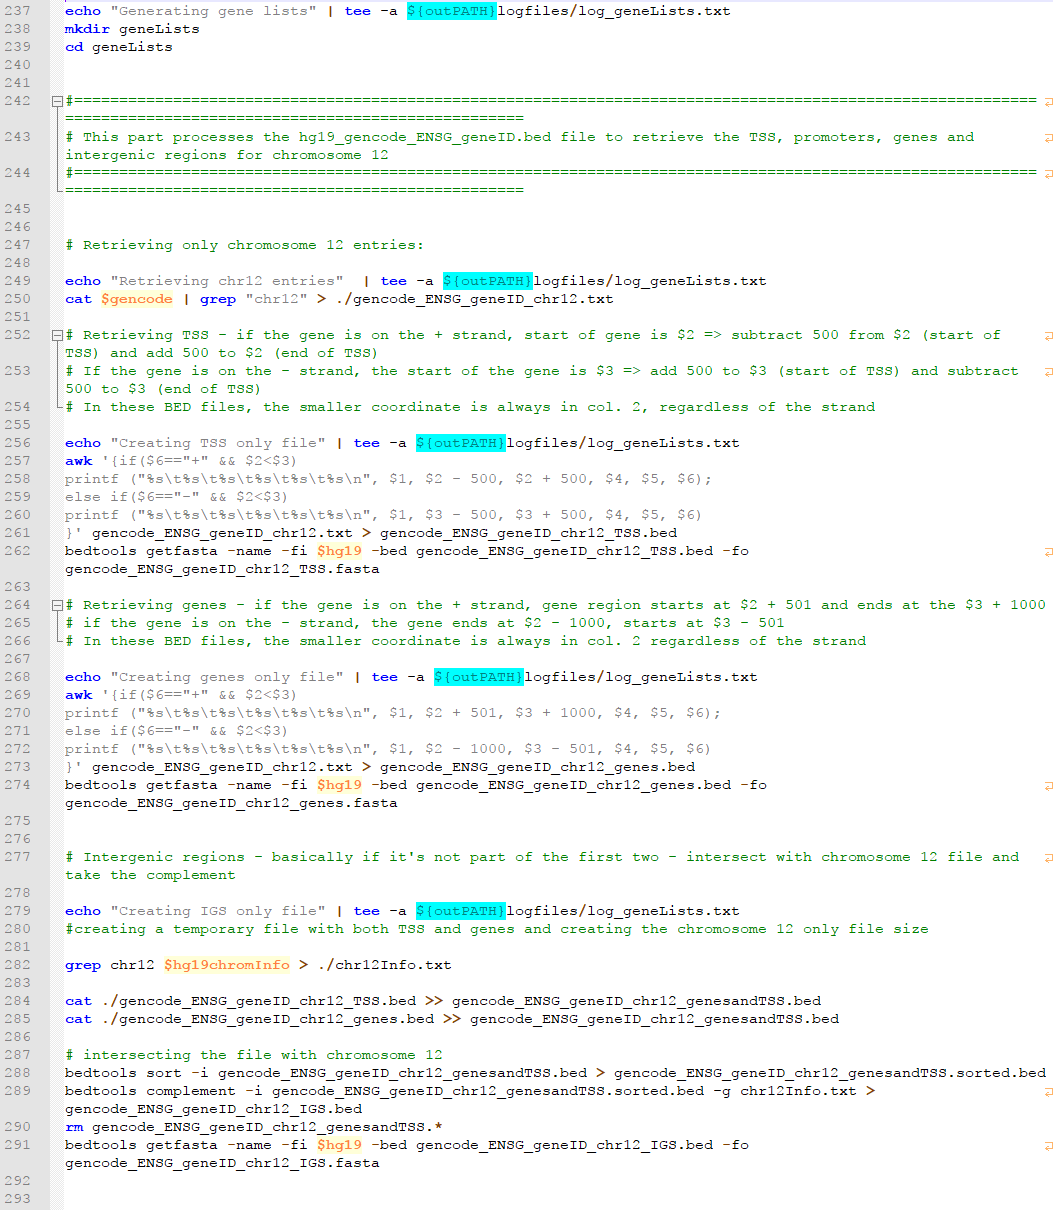
\includegraphics[scale=0.75]{geneLists1.PNG}

\subsection{Determining the distribution of high confidence peaks (summits) that fall into promoter, genes and intergenic sequences}
\noindent This entire code block is also under the same for loop which analyzes everything down to the TOMTOM step (therefore, it's far from the 'done' line)\\
 
\noindent 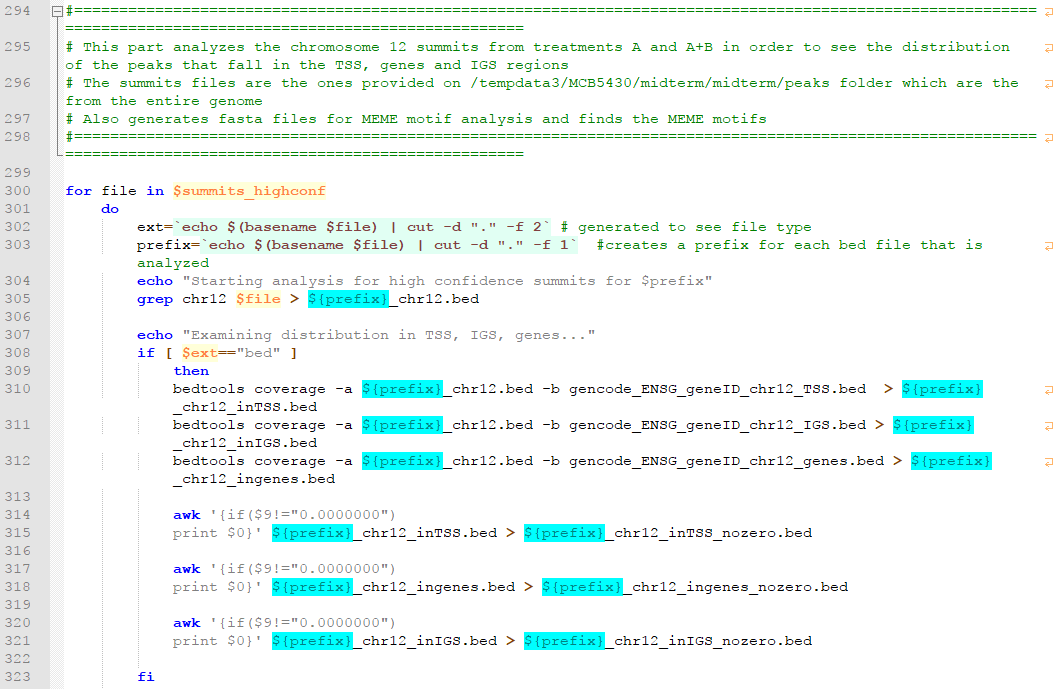
\includegraphics[scale=0.75]{Summits1.PNG}

\subsection{Summary table for distribution in genomic regions}
\noindent Table 2 contains a summary for the section 3.2 and for MAST and FIMO. The following example calculations show how the table was compiled:\\

\noindent \textbf{1. Grey rows: determining the distribution of high confidence peaks (summits) in different genome regions}\\

\noindent The numbers for overlapping summits for each genomic region are present in the columns starting with \#. The Total represents the sum of all summits falling in promoters, genes and intergenic sequences, and the percentages are calculated by dividing the number for each genomic region by the total number of summits:\\

\% in genes = ( \# in genes / \# Total ) * 100  \\

e.g. For Treatment A:

\noindent \% in genes = ( \# in genes / \# Total ) * 100\\
\% in genes = ( 411 / 1032 ) * 100\\
\% in genes = \textbf{39.82}.\\

\noindent \textbf{2. MAST outputs: determining how many peaks have motifs (peaks being broken down by different genome regions)}\\

\noindent Starting for example with \textit{treatment A intergenic regions}, 117 peaks have motif 1 and 137 peaks have motif 2. The total number of peaks with motifs for treatment A is therefore 117+137 = 254. To obtain the number of peaks without motifs, 254 was subtracted from the \textit{total peaks from intergenic regions} calculated in section 3.2 (in the grey bar):\\

\noindent \# peaks with no motifs in IGS = total \# peaks in IGS - total \# peaks w/ motifs in IGS\\
\# peaks with no motifs = 603 - 254 = \textbf{349}\\

\noindent To further calculate the percentages, I divided the number of peaks (having a certain motif in a certain genomic region) by the total number of peaks, regardless of genomic region. For example, for the treatment A intergenic regions for motif 1, the calculations were as following:\\

\noindent \% in IGS = ( \# in IGS / \# Total ) * 100\\
\% in IGS = (117 / 1032) * 100\\
\% in IGS = 11.34\\

\noindent This way, by looking at a genomic region percentages column, the white part of the table is essentially a breakdown of the grey row percentage. The table can be read, for example, like this: for treatment A, 58.43\% of peaks are in intergenic regions and out of 58.43 percents 11.34 of them have motif 1, 13.28 of them have motif 2 and 33.82 of them display no motif.\\


\noindent \footnotesize \textbf{Table 2.} Summary of MAST, FIMO and distribution of summits in different genomic regions. Certain features determined with either MAST, FIMO or bedtools are broken down by intergenic regions. Raw number of peaks as well as calculated percentages of the total are displayed. 
\flushleft \noindent 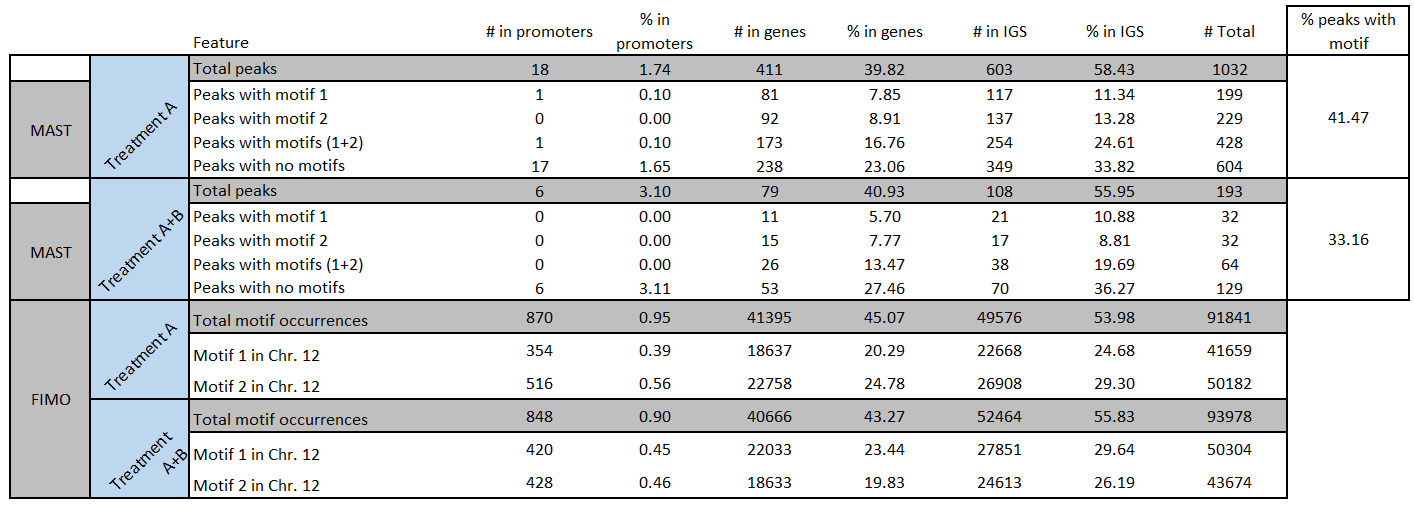
\includegraphics[scale=0.55]{Table2.PNG}

\normalsize
\subsection{TF preferences}
\noindent This transcription factor's preference for promoters or enhancers can be assessed by looking at the number of peaks falling in promoter regions and outside promoter regions. According to Table 2, for treatment A, 1.74\% of the summits are in the promoter regions, while 98.25\% are in genes and intergenic sequences. For treatment A+B, 3.10 \% of the summits are in the promoter regions, while 96.89\% of the summits are in genes and intergenic sequences. This means that the transcription factor has a strong preference to bind \textbf{enhancers}, rather than promoters.

\section{Identifying motifs under peaks}

\subsection{MEME}
\noindent 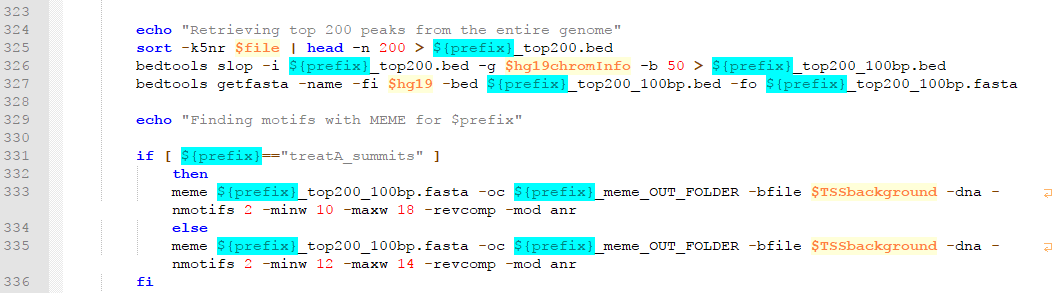
\includegraphics[scale=0.75]{MEME.PNG}

Using the code block above, the following motifs have been found (not displaying the reverse complements):

\subsection*{Treatment A}
\noindent \textbf{Motif 1:} \\
\noindent 
\includegraphics[scale=0.75]{A_meme1.PNG}\\
\noindent \textbf{Motif 2:} \\
\noindent 
\includegraphics[scale=0.75]{A_meme2.PNG}\\
\pagebreak
\subsection*{Treatment A+B}
\noindent \textbf{Motif 1:} \\
\noindent 
\includegraphics[scale=0.75]{AB_meme1.PNG} \\
\noindent \textbf{Motif 2:} \\
\noindent 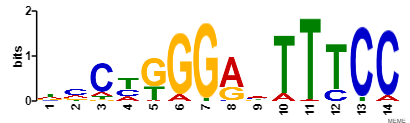
\includegraphics[scale=0.75]{AB_meme2.PNG} \\

\subsection{MAST}

\noindent 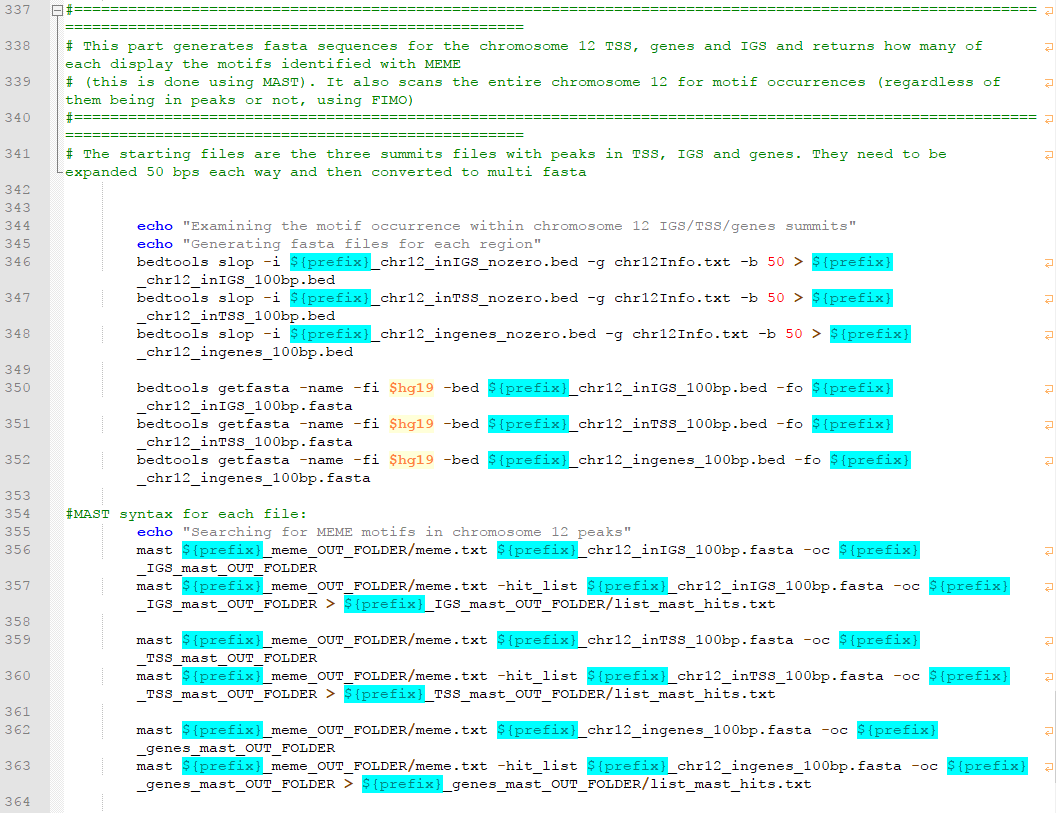
\includegraphics[scale=0.75]{MAST.PNG}


\subsection{FIMO}

\noindent 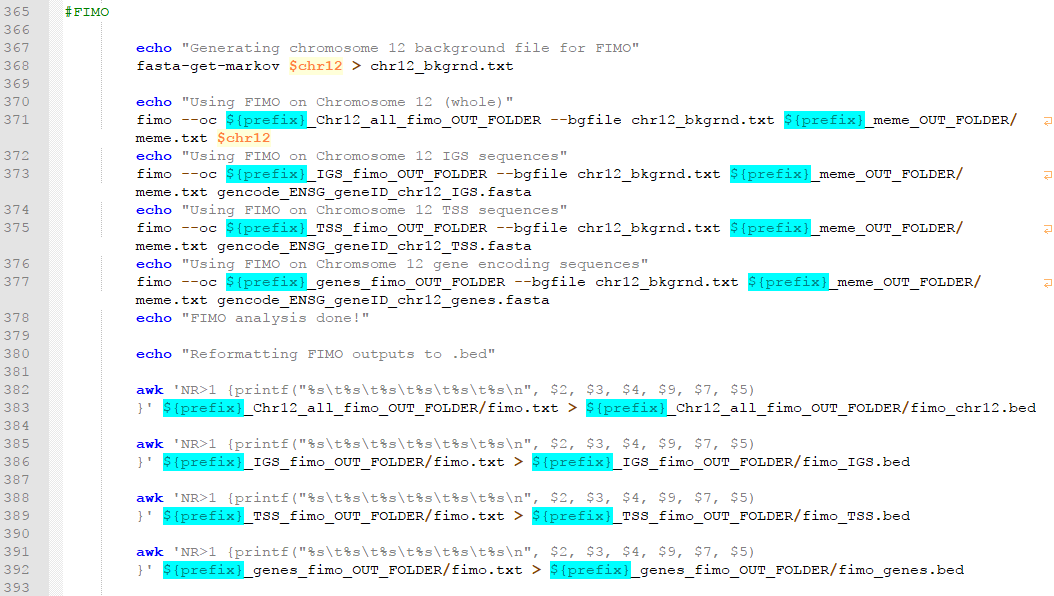
\includegraphics[scale=0.75]{FIMO.PNG}


\noindent In order to generate Table 2 statistics for FIMO, I used pipes to process the fimo.txt file and to find out out of the two motifs, how many occurrences are for motif 1 and how many are for motif 2, for each treatment. I then checked that the sum of the two is consistent with how many motif occurrences FIMO reports in the html file. E.g.

\begin{verbatim}
cat fimo.txt | cut -f 1 | grep 1 | wc -l    # for motif 1
\end{verbatim}

\begin{verbatim}
cat fimo.txt | cut -f 1 | grep 2 | wc -l	# for motif 2
\end{verbatim}

\textbf{Provide an explanation for why not all of your peaks have identified motifs.}\\

\noindent As observed in Table 2, only 41.47\% of the treatment A peaks display one of the two motifs identified using MEME. Likewise, for treatment A+B, only 33.16\% of the peaks have a motif. The reasons why we identify peaks without motif can be the following:\\
1. According to the chosen MEME options, I looked for the best two motifs only - there could be more than two and the percentages of peaks with a motif might be higher than these numbers.\\
2. Transcription factors, before any sequence specificity, have DNA binding domains, which causes them to be bound to DNA / chromatin even when not active.\\
3. Many transcription factors are ligand-dependent, which is a great way to finely modulate the regulation of a set of genes in a ligand concentration dependent manner. Different concentrations of ligands can result in various conformational changes for the transcription factors which can bind different DNA sequences in return.\\

\noindent \textbf{What do the results tell about the likelihood of the TF finding its motif?\\}

\noindent According to the FIMO outcomes (Table 2), there is an overwhelming amount of motif sequences the transcription factor could bind on Chromosome 12. By examining the percentages, for example in treatment A+B, it also appears that the proportion of peaks found in e.g. intergenic sequences (55.95\%) is about the same as the proportion of motifs found in intergenic sequences in the genome (53.98 and 55.83\% of motifs found on Chromosome 12 are in intergenic sequences).\\

\noindent This is obviously different from a situation where there would be very few motifs in the genome and the transcription factor would find them against all odds. This transcription factor seems to be \textit{statistically favored to encounter its motifs}, but the abundance of motifs makes it \textit{unlikely that the transcription factor finds its way to perform its function, e.g. upregulate a certain gene by binding to a particular enhancer}. We indeed observe it does not bind very many of these motifs, despite their abundance.

The reasons are plenty - it could be a matter of DNA accessibility (perhaps these motifs are tightly bound by histones which have repressive marks, especially in intergenic sequences), or it could be that the transcription factor generally lies at the end of a signaling cascade and its binding to the targets depends on other effector molecules as well, and not on the DNA sequence alone. This adds another degree of complexity which FIMO cannot account for.

\subsection{TomTom}

\noindent 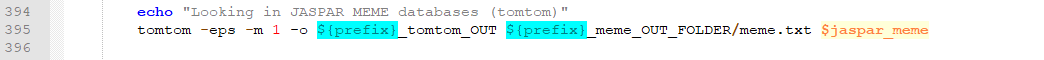
\includegraphics[scale=0.75]{tomtom.PNG}

\noindent According to the TomTom search, for treatment A, there are the following candidate transcription factors:
\begin{multicols}{2}
\begin{verbatim}
Name	MA0258.1				
Alt. Name	ESR2				
Database	jaspar.meme			
p-value	5.63649e-09

	Name	MA0112.1	
Alt. Name	ESR1
Database	jaspar.meme
p-value	8.99539e-09
\end{verbatim}
\end{multicols}

\noindent For treatment A+B, there are the following transcription factors:
\begin{multicols}{3}
\noindent \begin{verbatim}
Name	MA0112.2
Alt. Name	ESR1
Database	jaspar.meme
p-value	3.00279e-10

	Name	MA0258.1
Alt. Name	ESR2
Database	jaspar.meme
p-value	2.0445e-08

	Name	MA0066.1
Alt. Name	PPARG
Database	jaspar.meme
p-value	2.46812e-07
\end{verbatim}
\end{multicols}
\section{Final Question: What factor did Billy ChIP, and what were each of the treatments?}
\noindent From the TomTom hits above, one can confidently say that the antibody Billy did was against the Estrogen Receptor protein ESR1 or ESR2. According to the uniprot database, the following are known about the Estrogen Receptor ${^{[3]}}$ :\\
\vspace{0.5 cm}
\noindent ESR1 binds DNA as a homodimer and it can form heterodimers with ESR2 as well. Binding is followed by a phosphorylation event on both of the monomer subunits.\\
\vspace{0.5 cm}
Generally, ESR is stabilized by phosphorylation (and protected from proteosomal degradation). ESR activity is modulated by signaling pathway kinases that phosphorylate ESR1 as well as its interacting partners.\\
\vspace{0.5 cm}
ESR has three domains - a modulating N-terminal domain, a DNA binding domain (2 zinc fingers) and a C-terminal ligand binding domain. The N-terminal domain can transactivate in a ligand independent manner, while the C-terminal can transactivate in a ligand dependent manner. Transcription is canonically activated through the C-terminal domain by binding of estrogen. As a result of ligand binding, ESR1 associates with a network of coactivators and binds to estrogen responsive elements.\\
\vspace{0.5 cm}
Various mutations of ESR C-terminal domain are associated with disease. Several mutations result in estrogen resistance disease, where the variants have greatly reduced canonical activity in the presence of elevated estrogen levels. The non-classical activity of the mutants (through the estrogen independent domain) is greatly enhanced and this promotes tumor development and progression.$^{[1]}$\\
\vspace{0.5 cm}
As seen in Table 2, the total number of peaks for treatment A is 1032, while the number of peaks for treatment A+B is 193. An observation described in section 2.3 shows that the peaks in treatment A+B are a subset of treatment A, which means that the addition of B reagent results in a decreased binding of ESR 1 to the responsive elements. All things considered, for Chromsome 12 peaks, this is a 81.2\% decrease in binding.\\
\vspace{0.5 cm}							 
Assuming that the cell lines Billy has used have the wild type estrogen receptor, treatment A could be estrogen itself, while B can be anything that inhibits ESR1.\\
\vspace{0.5 cm}
One popular treatment for breast cancer cells with wild type ESR1 is an aromatase inhibitor. However, this is not a good choice because aromatase uses body levels of androgen hormones as a substrate and only the production of estrogen in a body context would be lowered.\\
\vspace{0.5 cm}
Another candidate for treatment B is tamoxifen, which is a competitor of estrogen in binding to ESR1 and an antagonist. However, tamoxifen binding to ESR1 still results in binding to DNA and repression of transcription, which in a ChIP-seq experiment would not result in differential binding of ESR1 to DNA - the peaks would still come up${^{[2]}}$.\\
\vspace{0.5 cm}
It is safe to assume interfering with phosphorylation will result in destabilizing the ESR1 homodimers or ESR1/2 heterodimers that can bind to DNA. Treatment A could be estrogen, while treatment B could be a kinase inhibitor which would show that even in the presence of estrogen, ESR1 cannot bind to the responsive elements. In addition, repressing phosphorylation in general affects the entire signaling pathway and prevents ESR1 interaction with DNA via both ligand dependent and independent domains.
\pagebreak
\section*{\footnotesize REFERENCES}

$[1]$ Jeselsohn R, Buchwalter G, De Angelis C, Brown M, Schiff R (2015) \textit{ESR1 mutations as a mechanism for acquired endocrine resistance in breast cancer} Nat Rev Clin Oncol. 12(10): 573–583.\\
\vspace{0.5 cm}
$[2]$ Wang DY, Fulthorpe R, Liss SN, Edwards EA (2004). \textit{Identification of Estrogen-Responsive Genes by Complementary Deoxyribonucleic Acid Microarray and Characterization of a Novel Early Estrogen-Induced Gene: EEIG1} Molecular Endocrinology, Volume 18, Issue 2, Pages 402–411.\\
\vspace{0.5 cm}
Internet resources:\\
$[3]$ www.uniprot.org/uniprot/P03372 (Retrieved on Nov. 5, 2017)

\end{document}
